\documentclass{tudelft-report}
\usepackage{natbib}
\usepackage{changes}

\usepackage{verbatim}
\usepackage{units}
\usepackage{mathtools}
\usepackage{amsmath}
\usepackage{amssymb}
\usepackage{graphicx}
\usepackage{wasysym}
\usepackage{siunitx}
\newcommand\bmmax{2}
\usepackage{bm}
\usepackage{xcolor}
\usepackage{bookmark}
\usepackage{tabularx}
\usepackage{microtype}
\usepackage{babel}

\renewcommand{\comment}[2]{#2}
% Uncomment the following line for paragraph descriptions to appear in the file.
% \renewcommand{\comment}{\paragraph}

% Parameters
\newcommand{\meff}{m_\text{eff}}

% Momentum operators
\newcommand{\kx}{k_x}
\newcommand{\ky}{k_y}

% Pauli matrices
\newcommand{\sigx}{\sigma_x}
\newcommand{\sigy}{\sigma_y}
\newcommand{\sigz}{\sigma_z}
\newcommand{\sigi}{\sigma_0}
\newcommand{\taux}{\tau_x}
\newcommand{\tauy}{\tau_y}
\newcommand{\tauz}{\tau_z}
\newcommand{\taui}{\tau_0}

% Operators
\DeclareMathOperator{\e}{e}
\DeclareMathOperator{\de}{d\!}
\DeclareMathOperator{\Tr}{Tr}
\DeclareMathOperator{\diag}{diag}
\DeclareMathOperator{\Res}{Res}
\DeclareMathOperator{\sgn}{sgn}
\DeclareMathOperator{\Pf}{Pf}
\DeclareMathOperator{\Det}{Det}
\DeclareMathOperator{\rank}{rank}
\DeclareMathOperator{\im}{Im}
\DeclareMathOperator{\re}{Re}

\begin{document}

%% Use Roman numerals for the page numbers of the title pages and table of
%% contents.
\frontmatter

\title[tudelft-white]{Improved isolation of Majorana bound states in zigzag-shaped junctions}
\subtitle[tudelft-black]{
% Optional subtitle
}
\author[tudelft-white]{T.M. Laeven}
% \affiliation{Technische Universiteit Delft}
\coverimage{images/cover.pdf}
% \coverimage{images/cover_onec.pdf}

\covertext[tudelft-white]{
    \textbf{
    % Cover Text
    } \\
    % possibly \\
    % spanning 
    % multiple 
    % lines
    % \vfill
    % ISBN 000-00-0000-000-0
}
\setpagecolor{tudelft-cyan}
\makecover


%% Include an optional title page.
% -*- root: ./report.tex -*-
\begin{titlepage}


\begin{center}

%% Insert the TU Delft logo at the bottom of the page.

%% Print the title in cyan.
{\makeatletter
\largetitlestyle\fontsize{64}{94}\selectfont\@title
%\largetitlestyle\color{tudelft-cyan}\Huge\@title
\makeatother}

%% Print the optional subtitle in black.
{\makeatletter
\ifx\@subtitle\undefined\else
    \bigskip
   {\tudsffamily\fontsize{22}{32}\selectfont\@subtitle}    
    %\titlefont\titleshape\LARGE\@subtitle
\fi
\makeatother}

\bigskip
\bigskip

by
%door

\bigskip
\bigskip

%% Print the name of the author.
{\makeatletter
%\largetitlefont\Large\bfseries\@author
\largetitlestyle\fontsize{26}{26}\selectfont\@author
\makeatother}

\bigskip
\bigskip

to obtain the degree of Master of Science
%ter verkrijging van de graad van Master of Science

at the Delft University of Technology,
%aan de Technische Universiteit Delft,

to be defended publicly on Tuesday February 12, 2019 at 14:30 AM.
%in het openbaar de verdedigen op dinsdag 1 januari om 10:00 uur.

\vfill

\begin{tabular}{lll}
    Student number: & 4247078 \\
    Project duration: & \multicolumn{2}{l}{March 1, 2018 -- November 28, 2018} \\
    Thesis committee: & dr.\ A.\ Akhmerov, & TU Delft \\
                      & Prof.\ dr.\ G.A.\ Steele, & TU Delft \\
                      & dr.\ M.T.\ Wimmer, & TU Delft \\
\end{tabular}
%% Only include the following lines if confidentiality is applicable.

\bigskip
\bigskip

The cover is a SEM image of a zigzag SNS junction fabricated and photographed by Fokko de Vries and Qingzhen Wang.
\bigskip

An electronic version of this thesis is available at \url{http://repository.tudelft.nl/}.
\end{center}

\begin{tikzpicture}[remember picture, overlay]
    \node at (current page.south)[anchor=south,inner sep=0pt]{
        
\includegraphics{cover/logo_black}
    };
\end{tikzpicture}

\end{titlepage}



\chapter*{Preface}
\setheader{Preface}

Preface\ldots

\begin{flushright}
{\makeatletter\itshape
    \@author \\
    Delft, January 2013
\makeatother}
\end{flushright}



\tableofcontents

%% Use Arabic numerals for the page numbers of the chapters.
\mainmatter

% -*- root: ./report.tex -*-
\chapter{Introduction}

\comment{The history of quantum computing and why QC is important}
	The idea to use coherent quantum states as a means to perform complex calculations first appeared in the beginning of the 80's.
	A handful of papers had already been published on the matter, when, during a keynote speech at the California Institute of Technology, Nobel laureate Richard Feynman suggested its importance with respect to physics simulations .
	To put his idea in very simple terms, calculating the quantum mechanical state of a system on a conventional computer scales exponentially with respect to the system size.
	By making a computer that is based on quantum states itself, and making a mapping between those states and the system you want to simulate, the idea is that this scaling becomes polynomial.
	Beyond its significance in physics simulations, quantum computers have been suggested to be used for other, perhaps more pragmatic tasks, including topics like cryptography, optimization and search algorithms.
	With the potential applications in mind, a lot of resources and effort has been put into realising such a quantum computer in recent years.
	Recently, apart from being a largely publicly funded effort, the private sector has also started to recognize the potential of the technology: large companies such as Microsoft, Google and IBM are investing into the development of a quantum computer.
	As of this moment, working quantum computers have been realized on a very small scale: calculations of meaningful scale are still not possible.

\comment{It is still an open question what the implementation for a qubit will be, but majorana's are one of the contenders}
	If we consider the evolution of the regular computer, we see that the technological/physical platform for the bit, something which can be in either of two states, 1 or 0, has been constantly changing.
	For the earliest computers, it was complex mechanical systems with gears and cogs.
	Then later, switching to electronics, binary states were implemented in the form of vacuum tubes, and later, up to today, it is the transistor which acts as the basic unit of computation.
	Similarly, because quantum computing is still in its infancy, there are still many contenders for what the underlying technology will be: what physical system will form the basis for the quantum bit, the qubit.
	Some of the current platforms for implementing a qubit being pursued are the transmon qubit, NV-centers, quantum dots, and Majorana bound states.
	Majorana bound states (MBSs) are a promising candidate to form the basis of a stable platform for topological quantum computing, and the specific way to create them are the topic of study in this manuscript.

\section{Majorana bound states as qubits}

	\comment{What are Majorana bound states}
	Majorana particles are particles that always come in pairs: one pair of Majorana's forms a single electronic state.
	Disambiguating electrons and holes into their Majorana counterparts is often analogized with splitting a complex number into its real and imaginary part.
	We write the Majorana operators in terms of the creation(annihilation) and annihilation(creation) operators of electrons(holes), respectively $\hat{c}^\dagger$ and $\hat{c}$:

	\begin{align}
		\hat{c} =  \frac{1}{2} \left( \gamma_1 - i\gamma_2 \right) && \hat{c}^\dagger = \frac{1}{2} \left( \gamma_1 + i\gamma_2 \right)
		\label{eq:intro_ferm2maj}
	\end{align}

	Inverting this, we get,
	\begin{align}
		\gamma_1 = \hat{c} + \hat{c}^\dagger && \gamma_2 = i \left( \hat{c} - \hat{c}^\dagger \right)
		\label{eq:intro_maj2ferm}
	\end{align}

	Note that the basic excitation is still a fermion (electron/hole); one cannot have just one Majorana, they always come in pairs.
	The idea is to create a system where we have a single pair of Majoranas which is seperated in space.

	A system in which this seperation can be accomplished was first proposed by Kitaev\cite{kitaev_unpaired_2001}.
	We consider a one dimensional chain of sites which can host a single fermion, and thus a pair of Majoranas.
	Suppose that the occupation of a site by a fermion comes at the cost of energy $\mu$.
	Also, we consider the situation where there is an interaction energy between neighboring sites: $t$ quantifies the energy cost of one site being occupied while the adjacent isn't, and $\Delta$ is the gain in energy if adjacent sites are both occupied or empty.
	This leads to the following Hamiltonian:

	\begin{equation}
		H = -\mu \sum_n \hat{c}_n^\dagger \hat{c}_n
		- t \sum_n \left( \hat{c}_{n+1}^\dagger \hat{c}_n +\text{h.c.} \right) 
		+ \Delta \sum_n \left( \hat{c}_n \hat{c}_{n+1} +\text{h.c.} \right) 
	\end{equation}

	Considering equation \eqref{eq:intro_ferm2maj} we can also write the Hamiltonian above using Majorana operators.
	In this way, we get a Hamiltonian describing pairing energies between Majoranas on adjacent sites.
	In figure, we discern two extremes:
	one is the situation where the pairing energy is minimal for Majorana pairs on the same site, the other is when the energy is minimal for pairing between of Majoranas from adjacent sites. 


	Borrowing the analogy from the online course Topology in Condensed Matter\cite{noauthor_topology_2015}, we can see an electron as a domino stone: the two ends, seperated by a line, each correspond to a Majorona particle.
	In the figure below\cite{noauthor_topology_2015}, the dominoes, and thus electrons, have been placed in a chain:\\
	
	\begin{centering}
	
\includegraphics[width=0.95\columnwidth]{images/majorana_dominoes}
	\end{centering}
	
	Corresponding to the system above, we have a Hamiltonian describing the physics of the system.

	In a regular system, the Majoranas on each end of stone are paired locally, as depicted in the figure below:\\

	\begin{centering}
	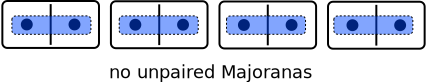
\includegraphics[width=0.95\columnwidth]{images/trivial_dominoes}
	\end{centering}
	
	Now suppose one would be able to shift the pairing, such that the Majoranas form pairs with the Majoranas on adjacent stones:\\

	\begin{centering}
	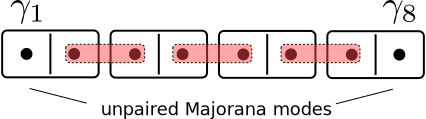
\includegraphics[width=0.95\columnwidth]{images/topological_dominoes}
	\end{centering}
	
	As is apparent from the above image, this would leave two unpaired Majoranas at the ends of the chain.
	This is the state we are interested in: the Majorana state, where two Majoranas are seperated in space.
	This physical seperation has the effect of not allowing simple local perturbations to disturb the system.

\section{Ways to make Majorana's: nanowires \& sns system}
	A realistic experimental implementation of Kitaev's model did not emerge until the similar works of Lutchyn et. al\cite{lutchyn_majorana_2010} and Oreg et. al\cite{ oreg_helical_2010}, where they proposed an experiment composed of a semiconducting nanowire deposited onto a superconductor.
	They predicted that, if the semiconductor has strong spin-orbit coupling, a magnetic field applied along the wire axis, as well as a carefully tuned chemical potential, Majoranas would appear at the ends of the nanowire.
	The experiment proved to be sufficiently practical to perform in the lab and the first signatures of Majorana bound states were found using the setup by Mourik et. al~\cite{mourik_signatures_2012}.

	For the same reasons Majoranas are inherently protected against decoherence, it is notoriously difficult to prove their existence.
	Perhaps the most direct way to detect their presence is through the observation of a so-called zero bias peak.
	When performing a tunneling conductance experiment, measuring the conductance through the nanowire, the zero-energy (with respect to the Fermi energy) Majorana state provides a resonant tunneling state when no bias is applied, appearing as a peak in conductance.
	There are however also other physical phenomena which can be responsible for such a conductance peak, and thus it is not unique to the Majorana state.

\section{Majoranas in a Josephson junction}
	\comment{Why are SNS junctions potentially better?}
	A more convincing case could be made if one could control the system in such a way that the presence of Majoranas can be turned on or off.
	This feature is realized in a relatively recent proposal by Pientka et. al\cite{pientka_topological_2017}, where, instead of a nanowire, a two-dimensional strip of semiconductor is used.
	On each side of the strip a superconductor is placed, forming a Josephson junction.
	Using the Josephson junction, one can use the supercurrent which flows between the two superconductors to control whether the system is in a topological phase (meaning it contains Majoranas), or not.
	The system has addition advantages, namely the system allows for Majorana's to be created at lower magnetic fields, the system is more compatible with convential semiconductor technology, and the Josephson junction allows for new ways to detect the topological phase of the system.

	% \comment{Current experimental progress}
	% Two papers that claimed they have observed signs of topological behavior.
	% Soft gap, questionable results.

	\comment{The challenges encountered}
	One of the biggest challenges in creating stable Majoranas is the appearance of a soft gap; where the gap in the density of states is greatly reduced for states with the momentum directed along the length of the strip.
	From a semiclassical perspective, these momenta correspond to long paths through the semiconductor without interruption by the superconductor.
	Additionally, these long trajectories have long flight times $\tau_f$ and equivalenly small Thouless energies $E_{\textrm{Th}}=\hbar / \tau_f$, resulting in a small gap. 
	Currently, proposed workarounds are low density or disorder~\cite{haim_double-edge_2018}, but both have drawbacks.


	We propose that the introduction of a zigzag-shaped modulation of the junction region leads to an increased topological gap, as well as a reduction of the Majorana coherence length.
	Furthermore, we hypothesize that the gap improvement is the result of the elimination of long trajectories
% -*- root: ./report.tex -*-

\chapter{Theory}
The topological quantum computer uses pairs of Majorana particles as its unit of computation (qubit).
In order to host Majorana modes in a system, one needs a material which has properties from a superconducting material, as well as from a semi-conducting material.
As this material does not seem to exist on its own, one creates a heterogeneous system.
I simple terms, this consists of a slab of superconductor and a strip of semiconductor.
By interfacing the two, one creates a region where all the necessary ingredients are present to realize Majorana's.

In this chapter, we first give a description of the normal (semi-conductor) and superconducting regions.
We then focus on what happens in a system where the two are interfaced.
Following that, we briefly explain what Majorana are, before introducing the implementation mainly relevant to this thesis.


\section{Normal region}
	Two important ingredients required for realizing Majorana fermions are strong spin-orbit coupling, and a strong interaction with the applied magnetic field.
	It is the normal conductor which brings these two physical effects to the mix.
	Note that the Hamiltonian of the normal region is the same for electrons and holes, except for the sign.
	The Hamiltonian terms provided in this section are relevant to the electron states.

    \subsection{Zeeman interaction}
    	The energy splitting of the two electron spin species due to magnetic field is called the Zeeman interaction.
    	It is modeled by:
    	\begin{equation}
    	H_\text{Z} = g \mu_B \vec{B} \cdot \vec{\sigma}
    	\end{equation}

    \subsection{Spin-orbit coupling}
	    An electron moving in an electric field will experience a small Zeeman field in its inertial frame as a relativistic effect~\cite{petersen_simple_2000}.
	    The resulting interaction, coupling the momentum and spin of electron, is known as spin orbit coupling.
	    Spin-orbit coupling can be approximated by adding a Rashba spin orbit coupling term in the Hamiltonian:
	    \begin{equation}
	    H_\text{Rashba} = \alpha (\ky \sigx - \kx \sigy) 
	    \end{equation}

\section{Superconducting region}
    The superconductor is responsible for ensuring particle-hole symmetry, as well as providing a `gapped' area in the bandstructure, isolating the zero-energy state.
    Superconductivity is a very complicated phenomenon, so we again provide only the background required for the understanding of this work.

    \subsection{Superconductivity}
		Superconductivity manifests itself as the complete lack of electrical resistance of a material.
		It is the result of the pairing of electrons close to the Fermi-energy, condensing into so-called Cooper pairs.
		The main parameter defining superconductivity is known as the superconducting order parameter, a complex number.
		The phase of this parameter is a macroscopic potential relative to ones choice of gauge.
		The magnitude of the superconducting order parameter, also referred to as the superconducting gap, quantifies the range around the Fermi-energy condensed into Cooper pairs.
		Because all electrons within a distance of the superconducting order parameter of the Fermi-energy are depleted in this way, charge transport only takes place via these quasiparticles.
		Scattering of these Cooper pairs is not allowed, resulting in perfect conduction.

		For the purpose of creating Majorana's, we are interested in two main aspects of superconductivity: the energy gap surrounding the Fermi energy (due to the depletion of states), and the electron-hole (/particle-hole) symmetry.
		We are thus not interested in the paired up electrons (Cooper pairs), and only wish to model the electronic (unpaired) modes.
		This can be achieved by modeling superconductivity with the Boguliubov de Gennes Hamiltonian:
		
		\begin{equation}
		\mathbf{H}_\text{BdG} = \begin{bmatrix} H & \Delta \\ \Delta^\dagger & H \end{bmatrix}
		\end{equation}

		The block matrix restricts the structure of the system in the electron-hole basis, and ensures particle-hole symmetry.
		For $\Delta \neq 0$ one indeed induces a identically sized gap in the spectrum.


\section{Normal-superconducting junctions}
	As mentioned, the interesting physics occur when a normal conductor is interfaced with a superconductor.
	A single interface between a normal conductor and a superconductor is known as a NS junction.
	When one creates a sandwich, superconductor - normal - superconducting, we speak of a SNS junction.
	Even not considering topological phases, which are only present if the normal regions meets certain conditions, both have interesting physics which will be discussed first.


	\subsection{Andreev scattering}
		At the interface between a normal and superconducting region, electrons with energies below the superconducting gap undergo Andreev scattering.
		The quasiclassical microscopic explanation for this is as follows.
		An electron in the normal region with energy below the superconducting gap, incident on the normal-superconductor (NS) interface, is retro-reflected as a hole.
		This phenomenon is known as Andreev scattering, and occurs due to the coupling of electrons in a superconductor.
		Although a single electron initially enters the superconductor, it draws another electron (with opposite momentum) into the superconductor: forming a Cooper pair.
		The drawn in electron leaves behind a hole in the normal conductor, which essentially backtracks the motion of the initial electron, hence the term retro-reflection.
		The same effect, but opposite in particle type, holds for a hole entering the superconductor.

	\subsection{Andreev bound states}
		If the normal region is finite in the direction normal to the NS/SN interface, Andreev bound states form.
		This is true for both SNS and SN junctions.
		Quasiclassically, one can imagine electrons (and holes) in the normal region, with energies below the gap, bouncing back and forth the system.
		The corresponding eigenstates have energies below the gap, and are thus bound to the normal region.

	\subsection{Josephson junctions and supercurrent}
		An important device in the field of condensed matter physics is the Josephson junction.
		A Josephson junction consists of a normal region sandwiched in between two superconductors (SNS junction).
		The resulting Andreev bound states exhibit interesting physics, making the Josephson junction an important device.

		Although superconducting phase is relative to the choice of gauge, the difference of phase between two superconductors is in fact a physical quantity.
		A difference in superconducting phase in a Josephson junction, results in a flow of current between the two superconductors: a supercurrent.
		The relationship between superconducting phase and current is known as the current-phase relationship, and is in the most simple case a sinosoid.
		This relationship can be exploited to control the phase difference: it is a matter of inducing a current.

		An important measure in a Josephson junction is the Thouless energy.
		In the context of this work, the Thouless energy is inversely proportional to the travel time of an electron in a system, without interacting with the superconductor(s).
		As an example of its relevance, in a SNS junction with magnetic field, if the Zeeman field has an energy comparable to the Thouless energy, as the electron traverses the system from supercondcutor to superconductor, the spin will be flipped.
		
\section{Topology and Majorana bound states}

	The Wikipedia definition of mathematical topology is as follows:
	
	\begin{quote}Topology can be formally defined as "the study of qualitative properties of certain objects (called topological spaces) that are invariant under a certain kind of transformation
	\cite{noauthor_topology_2018}
	\end{quote}

	Similarly, in condensed matter physics, topology refers to the study of properties of a system, which do not change within a particular range of parameters.
	Topology is relevant to the context of the system under study, because the emergence of seperated Majorana's is guaranteed within a continuous range of parameters.
	The precense of Majorana's is therefore \emph{topologically protected}, as they will be unpurturbed by variations of parameters, within a certain range.
	For an infinite system, the system is said to be topological if Majorana's would emerge if the system is cut to finite length.
	The system is trivial if the converse is true.

	\subsection{Majorana bound states}
		We will give a very pragmatic description of Majorana bound states, insofar their relevance to this work.

		The Majorana state is a superposition of electrons and holes, and is its own anti-particle: exchanging electrons and holes yields the same state.
		The Majorana state carries no spin, charge, or energy, giving almost no degrees of freedom for it to interact with the environment.
		The Majorana state constitutes a single fermion, but is comprised of two Majorana's.
		In a finite, topological system, these two Majorana's are physically seperated, appearing at the edges.

		The lack of interaction, as well as the physical seperation of the state, makes it very robust against perturbations, but also difficult to detect.
		Luckily, the state's presence itself is measurable: the availability of a state contributes to the conduction at that energy.
		When measuring the conduction through a system with Majorana's present, one should thus encounter a rise in the conductance at zero energy: the zero bias peak.

	\subsection{Decay/Coherence length}
		The decay or coherence length of a Majorana pair is an important measure signifying the seperation of the two half-particles.
		A decay length larger or of equal size to the system dimensions will lead to overlap of the Majorana's, diminishing the desired robustness of the state.
		An overlap of the Majorana's will in fact lead to the system having a non-zero energy, its magnitude depending on the amount of overlap.
		A crude estimation of the size of an individual Majorana is:
		\begin{equation}
			\xi = \hbar \frac{v_\text{F}}{\Delta}
		\end{equation}

	\subsection{Topological gap}
		The topological gap is defined as the energy gap between the Majorana state -- conveniently located at zero energy -- and the first available state.
		It's magnitude governs the protection of the system against perturbations causing the system to be lifted out of its ground state: the Majorana state.

\section{Two dimensional platform for Majoranas}

	\begin{figure}[!htb]
	\centering
	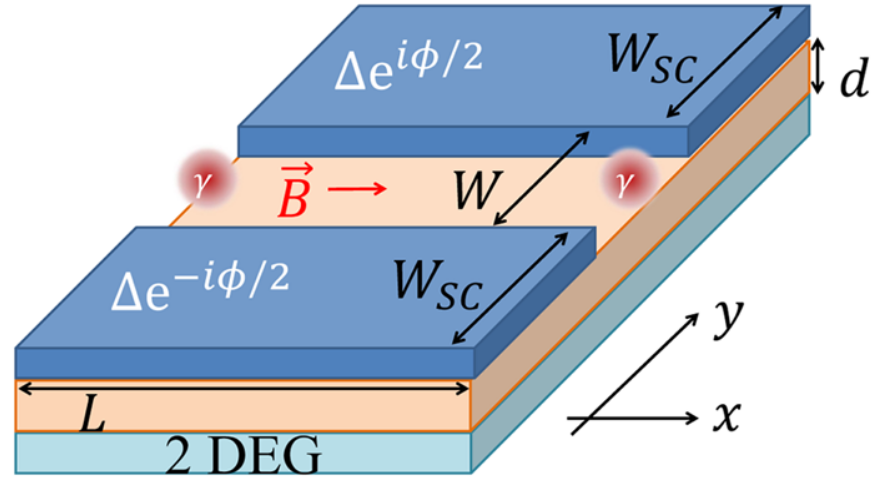
\includegraphics[width=0.5\columnwidth]{figures/pientka_system}
	\caption{System overview. Source\cite{pientka_topological_2017}}
	\label{fig:pientka_system}
	\end{figure}

	The earliest devices used to create a seperated pair of Majorana's were nanowires deposited onto a slab of superconducting material.
	A relatively new proposal is that of creating Majorana's in a planar Josephson junction~\cite{pientka_topological_2017}.
	An advantage of this system is that the phase difference between the superconductors can be used as a knob to switch the system from the topological state to the trivial state. 
	In addition, the presence of the second superconductor increases the topological gap of the system due to the proximity effect.

			

	\subsection{Phase diagram}
		As mentioned, the superconducting phase difference plays a critical role in the physics of the device.
		The topological phase diagram, as a function of magnetic field and superconducting phase, is depicted in Fig. \ref{fig:pientka_phase_diagram}.
		Without normal reflection (perfect Andreev reflection), the diagram has a diamond-like shape.
		The system is always topological when the superconducting phase is $pi$, or when the magnetic field is tuned to $(2N-1)$ times the Thouless energy (With exception of the corners of the diamonds).
		
		\begin{figure}[!htb]
		\centering
		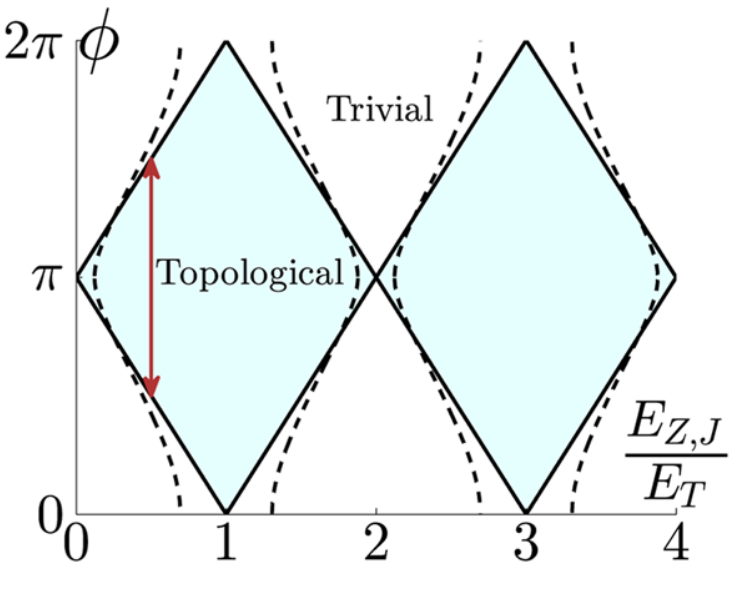
\includegraphics[width=0.5\columnwidth]{figures/pientka_phase_diagram}
		\caption{Phase vs. Magnetic field. Source\cite{pientka_topological_2017}}
		\label{fig:pientka_phase_diagram}
		\end{figure}
			
	\subsection{Bandstructure of a typical system}

% -*- root: ./report.tex -*-
\chapter{Methods}

\section{Tight binding simulation}

	\begin{figure}[!htb]
	\centering
	\includegraphics[width=0.95\columnwidth]{figures/kwant_system}
	\caption{Figure of different examples of simulated systems in Kwant.
	Lattice spacing is made smaller to make the discretization visible.
	The two golden regions are both superconducting, but differ in phase.
	The blue and black regions form the semiconductor, but the black region has an optional potential offset to model an imperfect interface, increasing the amount of normal reflection.}
	\label{fig:kwant_system}
	\end{figure}

	\comment{We use kwant to make systems and extract the eigenstates}
	We use a tight-binding model, implemented using Kwant, to simulate various properties of the system.
	The model consists of a two-dimensional square lattice of sites.
	Each site has two orbitals: spin and electron-hole.
	There are four different types of sites (and thus four different Hamiltonians): the top superconductor, the bottom superconductor, the normal region, and a normal region with a variable potential offset, forming a barrier to simulated an imperfect NS interface.
	A schematic of such kwant systems is depicted in Fig.~\ref{fig:kwant_system}.
	After the system is specified, we can extract the total Hamiltonian of the system, allowing analysis of the eigenstates.

	\comment{We extract the gap by either taking the lowest energy state for an infinite system, or the difference between the lowest two eigenstates.}
	

\comment{We propose a method to verify that elimination of long trajectories is responsible for the increased topological gap in a zigzag system.}
\section{Quasiclassical estimation of the topological gap}
	\comment{To compute the effect of cutoff consider a single segment of the zigzag and obtain the spectrum analytically (this allows to use translation invariance).}
	In order to establish that the elimination of long trajectories is the driving mechanism behind the order of magnitude gap improvement, we use an analytical approach.
	We estimate the gap of the zigzag system by the minimum energy occuring in the Andreev spectrum of a single (diagonal) segment of zigzag.
	The spectrum of the zigzag segment we define as the spectrum of an infinite ribbon SNS junction with tilted-magnetic field. 
	The finite length of the segment is modeled by not including momenta corresponding to long trajectories when taking the minimum over the spectrum.

	\comment{The spectrum is derived using a scattering matrix, and we consider multiple ways to eliminate long trajectory momenta.}

	Estimating the gap is a two-step process: derivation of the Andreev spectrum, and taking the minimum energy over a particular set of allowed momenta.
	The first is derived using scattering matrix formalism and the Andreev bound state condition\cite{beenakker1991universal, sticlet_robustness_2017}.
	The second step is mostly trivial, but the difficulty lies with identifying the set of allowed  momenta to take the minimum over.


	\subsection{Analytical estimate of Andreev spectrum for a straight junction}
		
		We derive the spectrum by calculating the scattering matrix for the normal region and applying the Andreev bound state condition for the short junction limit\cite{beenakker1991universal, sticlet_robustness_2017}. 
		The short junction limit is valid for [TODO: WHEN IS THE SHORT JUNCTION LIMIT VALID]
		For deriviation of the scattering matrix, we neglect SOI in the transverse direction, which is valid for $W<l_\text{so}$.

		\subsubsection{Derivation of the scattering matrix}

			\begin{figure}[!htb]
			\centering
			\includegraphics[width=0.75\columnwidth]{images/scattering}
			\caption{Basis for scattering matrix. 
			The `S' region corresponds to the superconductor Hamiltonian without the superconducting term, Eq.~\eqref{eq:ham_smat_superconducting}, `N' to the normal region, Eq.~\eqref{eq:ham_smat_normal}. 
			The coefficients represent the amplitude of the modes present in the system, at a particular energy.
			The different color arrows correspond to the two different spinors in each region.
			For example, $a_{1,L}$ is the amplitude of the rightmoving incoming mode, $\vec{\psi}_1 \exp\left(i k_{1,L} x\right)$}
			\label{fig:scattering}
			\end{figure}
			
			\begin{align}
			H_\text{N} &= \left[ \frac{\hbar^2}{2 \meff} \left(\kx^2 + \ky^2\right) -\mu_n\right]\sigi +
						 \alpha \kx \sigy +
						 E_z \left[ \cos(\theta) \sigx + \sin(\theta) \sigy \right]
			\label{eq:ham_smat_normal} \\
			H_\text{S} &= \left[\frac{\hbar^2}{2 \meff} \left(\kx^2 + \ky^2\right) -\mu_s\right]\sigi
			\label{eq:ham_smat_superconducting}
			\end{align}
			
			We consider the scattering region as depicted in Fig. \ref{fig:scattering}.
			There are three regions in the system, one normal system (N), with Hamiltonian given by Eq.~\eqref{eq:ham_smat_superconducting}, and two superconducting regions (S), with Hamiltonian given by Eq.~\eqref{eq:ham_smat_superconducting}.
			Not that Eq.~\eqref{eq:ham_smat_superconducting} region does not include the superconducting term ($\Delta \tau_y$), because we implement Andreev reflection seperately: this way we avoid doubling (electron and hole) the dimensionality of the problem.
			We set the energy of the system, and find the planar waves propogating in each region.
			Because the plane waves can go in two directions, and the additional degree of freedom introduced due to spin, each region has four propogating waves.
			The idea of the scattering matrix is to set the vector $\vec{a}$, containing the amplitudes of the planar waves coming in to the scattering region, and find the amplitudes of the modes exiting the scattering region.
			This is captured by a system of linear equations, displayed in Eq.~\eqref{eq:scattering_matrix_problem}
			
			\begin{equation}
			\begin{bmatrix} 
			b_{1,L}\\
			b_{2,L}\\
			b_{1,R}\\
			b_{2,R}
			\end{bmatrix} 
			= S_\text{sns}(\epsilon) \cdot 
			\begin{bmatrix} 
			a_{1,L}\\
			a_{2,L}\\
			a_{1,R}\\
			a_{2,R}
			\end{bmatrix}
			\label{eq:scattering_matrix_problem}
			\end{equation}

			In order to find the coefficients of the matrix $S_\text{sns}(\epsilon)$, we take the wavefunction $u(x)$ and apply the boundary equations (continuity and flux conservation): specified in Eqs.~\eqref{eq:scattering_equations} through \eqref{eq:scattering_boundary_eqs}.
			Note that because we neglect spin-orbit coupling in the x-direction, the velocity operator $\hat{\mathbf{v}}$ can be simplified to the first derivative.
			Although omitted to keep the expression compact, the momenta $k_i, q$ and spinors $\vec{\Psi_{i, L/R}}$ are energy dependent.

			\begin{align}
				&u(x) = 
				\begin{cases}
				u_L(x) = a_{1,L} \vec{\Psi} _{s,1} \exp (i q y) + a_{2,L} \vec{\Psi} _{s,2} \exp (i q y) + b_{1,L} \vec{\Psi} _{s,1} \exp (-i q y) + b_{2,L} \vec{\Psi} _{s,2} \exp (-i q y)  & x \leq 0\\
				u_m(x) = d_{1,l} \vec{\Psi} _{n,1} \exp \left(-i k_1 y\right) + d_{1,r} \vec{\Psi} _{n,1} \exp \left(i k_1 y\right) + d_{2,l} \vec{\Psi} _{n,2} \exp \left(-i k_2 y\right) + d_{2,r} \vec{\Psi} _{n,2} \exp \left(i k_2 y\right)  & 0 \geq x \leq W\\
				u_R(x) = a_{1,R} \vec{\Psi} _{s,1} \exp (-i q y) + a_{2,R} \vec{\Psi} _{s,2} \exp (-i q y) + b_{1,R} \vec{\Psi} _{s,1} \exp (i q y) + b_{2,R} \vec{\Psi} _{s,2} \exp (i q y)  & W \geq x
				\end{cases}
				\label{eq:scattering_equations}
			\end{align}
				
			Where $a_{i, L/R}$ are the coefficients of the incoming modes, $b_{i, L/R}$ are those of the outgoing modes, and $d_{i, l/r}$ are the modes in the middle region: see Fig.\ref{fig:scattering}.
			The symbols $\vec{\Psi}_{n/s, i}$ and $k_i, q$ are respectively the spinors and corresponding momenta belonging to each region.
			Both are energy dependent.\\

			The boundary conditions are,
			\begin{align}
				& u(x) \text{ is continuous}\\
				&\hat{\mathbf{v}} u(x) \text{ is continuous, where $\hat{\mathbf{v}}$ is the velocity operator}\label{eq:scattering_boundary_eqs}
			\end{align}

			To solve the system analytically, we use the Short Junction limit: we set the energy to zero.
			By applying the boundary conditions and solving the resulting linear system of equations, the resulting solution is given by Eqs.~\eqref{eq:smatrix} through ~\eqref{eq:momenta_short_junction}.
			\emph{Important note: In order to use the Andreev bound state condition, the scattering matrix must be in the [TODO: NAME OF BASIS] basis. This basis transformation has already been applied in Eqs. ~\eqref{eq:smatrix} through ~\eqref{eq:momenta_short_junction}}\\
			
			Scattering matrix, in block matrix format:
			\begin{align}
			\label{eq:smatrix}
		    S &= \left(
		    \begin{array}{rr}
		    r_{ll}&t_{rl}\\
		    t_{lr}&r_{rr}\\
		    \end{array}
		    \right) =
		    \left(
		    \begin{array}{rr}
		    \beta_+ & e^{-i q W} \beta_-\\
		    e^{-i q W} \beta_- & e^{-2 i q W} \beta_+\\
		    \end{array}
		    \right)
		    \\
		    \beta_\pm &= \left(
		    \begin{array}{rr}
		    e^{i \nu_{\arg}}\left(\omega^\pm_1 - \omega^\pm_2\right) & (\omega^\pm _1 + \omega^\pm _2)\\
		    -(\omega^\pm _1 + \omega^\pm _2) & e^{-i \nu _{\arg }} \left(\omega^\pm _2 - \omega^\pm _1\right)\\
		    \end{array}
		    \right)\\
		    \omega^\pm_j &= \frac{1}{4} \left(\gamma _{j} \pm \delta _{j}\right)
			\end{align}

			Subexpressions:
			\begin{align}
			    \gamma_j &= \frac{q+i k_{j} \tan \left(\frac{W k_{j}}{2}\right)}{q-i k_{j} \tan \left(\frac{W k_{j}}{2}\right)} \\
			    \delta_j &= \frac{q-i k_{j} \cot \left(\frac{W k_{j}}{2}\right)}{q+i k_{j} \cot \left(\frac{W k_{j}}{2}\right)}\\
			    e^{i \nu_{\arg}} &= \frac{E_\text{z} e^{i \theta }-i \alpha  k_x}{\sqrt{E_\text{z}^2+\alpha  k_x \left(\alpha  k_x-2 E_\text{z} \sin (\theta )\right)}}
			\end{align}

			Momenta:
			\begin{align}
			    q &= \left[ \frac{2 m_\ast}{\hbar ^2}\mu_s - k_x^2 \right]^\frac{1}{2}\\
			    k_1 &= \left[ \frac{2 m_\ast}{\hbar^2} \left(\mu_n-\sqrt{E_z^2-2 \alpha  E_z \sin (\theta ) k_x+\alpha ^2 k_x^2}\right) - k_x^2 \right]^\frac{1}{2}\\
			    k_2 &= \left[ \frac{2 m_\ast}{\hbar^2} \left(\mu_n+\sqrt{E_z^2-2 \alpha  E_z \sin (\theta ) k_x+\alpha ^2 k_x^2}\right) - k_x^2 \right]^\frac{1}{2}
			\label{eq:momenta_short_junction}
			\end{align}

		\subsubsection{Resulting spectrum}
			In order to get the spectrum from the S-matrix [Eq.~\eqref{eq:smatrix}] we use the main result from Ref.~\cite{beenakker1991universal} and start with a determinantal equation for the bound state energies in a SNS-junction:

			\begin{equation}
			\det\left[1+\alpha^{2}\left(E\right)r^{*}S_{e}\left(E,\bm{k}\right)rS_{e}^{*}\left(-E,-\bm{k}\right)\right]=0
			\end{equation}

			We rewrite this as a characteristic polynomial problem $\det\left[A-\lambda I\right]=0$, as

			\begin{equation}
			\det\left[r^{*}S_{e}\left(E,\bm{k}\right)rS_{e}^{*}\left(-E,-\bm{k}\right)-\frac{-1}{\alpha^{2}\left(E\right)}I\right]=0
			\end{equation}

			with
			\begin{equation}
			\lambda=-\frac{1}{\alpha^{2}\left(E\right)},\;A=r^{*}S_{e}\left(E,\bm{k}\right)rS_{e}^{*}\left(-E,-\bm{k}\right).
			\end{equation}

			Where $\lambda_i$ are the eigenvalues of $A$.
			Inverting $\alpha\left(E\right)\equiv\exp\left(-i\arccos\left(E/\Delta\right)\right)$ yields $\frac{E}{\Delta}=\frac{\alpha^{2}+1}{2\alpha}=\frac{1}{2}\left(\alpha+\alpha^{-1}\right)=\textrm{Re}(\alpha)$, where the last equality holds because $\alpha$ is unitary.
			Then, since $\alpha$ is only defined in the positive imaginary plane, the energies are $\frac{E_{i}}{\Delta}=\textrm{Re}\left(\sqrt{-1/\lambda_{i}}\right)$ where we take the root which has a positive imaginary part.
			Using this result and Eq.~\eqref{eq:smatrix}, we numerically find the Andreev spectrum.

	\subsection{Eliminating long trajectories}

		\begin{figure}[!htb]
		\centering
		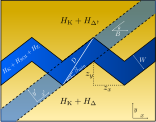
\includegraphics[width=0.75\columnwidth]{images/zigzag_methods.pdf}
		\caption{Schematic of the system, along with relevant dimensions, and the quasiclassical approach.
		The $x^\prime, y^\prime$ axis depicts the rotated frame for the quasiclassical estimate.
		The white trajectory indicates the estimate taken for the longest trajectory allowed by a zigzag.
		\label{fig:zigzag_methods}}
		\end{figure}

		\comment{We make an analogy between the cutoff of long trajectories to the cutoff of high momenta.}
		We hypothesize that the increase of the topological gap in a zigzag is due to the cutoff of modes on the Fermi surface with long trajectories.
		In order to make substantiate that this is indeed the driving mechanism behind the improvement, we propose an analogy using the bandstructure of a regular SNS junction.

		\comment{We map the zigzag to an infinite SNS junction with tilted magnetic field and a range of forbidden momenta.}
		We essentially take a single diagonal section of a zigzag, and map it to a normal, infinite SNS junction.
		We assume that the zigzag is shaped such that there is no straight trajectory possible through the system anymore.
		The system is depicted in Fig.~\ref{fig:zigzag_methods}, along with the set of axes with $x^\prime$ and $y^\prime$.
		Note that the magnetic field has an angle $\theta$ with respect to the $x^\prime$ axis.
		We identify trajectories cut off by the zigzag with a particular range of forbidden momenta.
		By then analysing the bandstructure of this infinite SNS junction, ignoring the forbidden momenta, we can give an estimate the resulting gap of the device.
		As the system is only momentum localized in the $x$ direction (the translationally invariant direction), we only control $\kx$.
		Denoting the set of allowed momenta by $\Omega$, the equation for the estimated topological gap becomes,
		
		\begin{equation}
			\Delta_\text{topological} = \min_{\kx\in\Omega} \left\rvert E(\kx) \right\rvert
			\label{eq:definition_gap}
		\end{equation}
		
		\comment{We first link the long trajectories to a maximum allowed angle.}
		In the infinite system, the long trajectories have a small angle with respect to the $x^\prime$ axis.
		By defining a minimum angle, we thus can filter out the long trajectories.
		We define this angle $\beta\text{min}$ by identifying it with the angle of the longest trajectory from one side of the superconductor to the other: see Fig.~\ref{fig:zigzag_methods}.
		Note that longer trajectories exist, by `grazing' the concave corners of the zigzag.
		We suspect that this `grazing' leads to physics which cannot be captured in this simple model, and we thus choose to restrict this method for systems where the chosen trajectory is indeed a good approximation of the longest path.

        We identify the momentum with its angle by defining it through the reciprocal of the component velocities, given by Eq.~\eqref{eq:methods_angle_of_state}. Note that $k_1$ and $k_2$ are the momenta as defined in Eq.~\eqref{eq:momenta_short_junction}.

        \begin{equation}
        \tan (\beta) = \frac{v_y}{v_x}\bigr{\rvert_{E=E_F}} = \frac{ \frac{\de E}{\de k_y} }{ \frac{\de E}{\de k_x} } \Biggr\rvert_{E=E_F}=
        \begin{cases}
        \frac{\hbar ^2 k_1}{\frac{\alpha  \meff \left(\alpha  k_x-\text{Ez} \sin (\theta )\right)}{\sqrt{\text{Ez}^2+\alpha  k_x \left(\alpha  k_x-2 \text{Ez} \sin (\theta )\right)}}+\hbar ^2 k_x} & \text{band 1}\\
        \frac{\hbar ^2 k_2}{\frac{\alpha  \meff \left(\text{Ez} \sin (\theta )-\alpha  k_x\right)}{\sqrt{\text{Ez}^2+\alpha  k_x \left(\alpha  k_x-2 \text{Ez} \sin (\theta )\right)}}+\hbar ^2 k_x} & \text{band 2}
        \end{cases}
        \label{eq:methods_angle_of_state}
        \end{equation}
		
        We estimate the restriction of the domain for the momentum by geometrically calculating the minimum angle, as depicted in Fig.\ref{fig:zigzag_methods}. The result:

        \begin{align}
        	\tan \left(\beta_\text{min} \right) = \frac{W}{\sqrt{D^2 - W^2}} \label{eq:beta_min}\\
        	D = \sqrt{z_x^2 + \left(z_y + W \sqrt{1 + \left(\frac{z_y}{z_x}\right)^2}\right)^2} \nonumber
        \end{align}

        The condition for the restricted momentum becomes:
        \begin{equation}
        	\tan \left(\beta\right) \geq \tan \left(\beta_\text{min}\right)
        	\label{eq:restriction_momentum}
        \end{equation}
% -*- root: ./report.tex -*-
\chapter{Results \& Discussion}\label{chap:results}
		In this chapter, we show how some properties of the system change by the introduction of a zigzag geometry.
		Additionally, we attempt to isolate the mechanism behind the improved properties by estimating the gap size through the quasiclassical model introduced in chapter \ref{chap:methods}.

	\comment{Introduction of a zigzag opens up the gap, creates a more stable topological phase diagram, and decreases coherence length of Majoranas}
	\section{Increased isolation and stability of the Majorana state}

		\comment{We see that the introduction of a zigzag leads to a reduction of the gap}
		\subsection{Gap/bandstructure as a function of zigzagginess}

			\begin{figure}[!htb]
			\centering
			\includegraphics[width=0.55\columnwidth]{figures/bandstructures}
			\caption{Figure of the bandstuctures corresponding to the system in Fig.~\ref{fig:zigzag_methods}.
			Blue lines correspond to $\phi=0$, $B=0$, red lines to $\phi=\pi$, $B = 1$.
			Thre three subplots are for different amplitudes of zigzag: (a) $z_y=0$, (b) $z_y=\frac{W}{4}$, and (c) $z_y=\frac{W}{2}$, where $W=200$\si{\nm} is the junction width.
			We observe that once there are no more straight trajectories inside the junction (when $z_y=\frac{W}{2}$) the spectrum becomes most insensitive to the momentum $k_x$.
			The value of the remaining parameters are $\alpha=20$ \si{\milli \eV \nm}, $g=26$, $\meff=0.02$\si{\electronmass}, $\mu=20$ \si{\milli \eV}, $\Delta=1$ \si{\milli \eV}.
			\label{fig:bandstuctures}}
			\end{figure}

			\comment{We calculate the bandstructure for varying amount of zigzag.}
			We implement a tight-binding version of the model described in section \ref{sec:physical_picture}.
			In figure~\ref{fig:bandstuctures}, the bandstructure for saw-toothed zigzag systems [Fig.~\ref{fig:zigzag_methods}] with varying amplitude is displayed.
			Because the zigzag has to be modelled using a supercell, we see a folded bandstructure.
			For comparison's sake, we take the same cell size for the ribbon structure, so the bandstructure folds in the same way.

			\comment{The band structures show that modulation of the geometry increases the gap by an order of magnitude, as well as reduce the group velocity.}
			The introduction of a zigzag has a striking effect: the bands flatten out, and more importantly, the gap size increases more than an order of magnitude.
			This increase happens because the modes where the gap is the smallest when the momentum almost entirely focuses along the strip ($k_x=k_F$), are cut off in a zigzag geometry.
			There is also a significant reduction of the group velocity where in Fig.~\ref{fig:bandstuctures} (c) the bands are nearly completely flat.
			The size of the gap, together with the velocity, directly relate to the Majorana coherence length (Eq.~\eqref{eq:majorana_coherence_length}), which we discuss in the following section.

			\comment{The introduction of an SN interface at many angles also increases performance.}
			Finally, in the presence of normal reflection, due to the availability of NS interfaces at a wide range of slopes, a zigzag system has an increased effective transmission.
			In a zigzag system, the normally reflected part of a wavefunction will eventually intersect a surface with which it is nearly perpendicular to.
			The transparency of the NS interface thus improves for non-transversal modes.

		\comment{Introduction of a zigzag leads to localization of the Majoranas}
		\subsection{Majorana decay length}

			\comment{We calculate the lowest eigenfunction and plot the density.}
			Using the tight-binding package Kwant~\cite{groth_kwant:_2014}, we model a finite system to compute the Majorana wave function density for different geometries; ribbon, zigzag, parallel curve, and vertically offset sinusoids.
			In figure~\ref{fig:wavefunctions} displays the wavefunctions superimposed upon their respective geometry including the corresponding Majorana energies $E_M$, as well as $E_1$: the energies corresponding to the next lowest state.

			\begin{figure}[!htb]
			\centering
			\includegraphics[width=0.55\columnwidth]{figures/wavefunctions}
			\caption{Wavefunctions for different sizes and geometries.
			With (a) a straight system, (b) a zigzag system, (c) a system where lines parallel to a sinusoid defines the normal region, and (d) a system with vertically offset sinusoids.
			Inside the figure, we indicate the Majorana length (or coherence length) $\lambda_\textrm{M}$ and the topological energy gap $E_\textrm{gap}$.
			We observe that $\xi$ for (a) is orders of magnitude longer and $E_\textrm{gap} = E_\textrm{1} - E_M$ orders of magnitude smaller than for (b), (c), and (d), meaning that the details of the geometry do not matter for the improvements to occur.
			\label{fig:wavefunctions}}
			\end{figure}

			\comment{In a straight system, the Majoranas are very poorly localized.}
			For the ribbon system [Fig.~\ref{fig:wavefunction}(a)], we see that the decay of the density is long compared to the system size.
			We see that the wavefunction extends to the centre of the system, not showing the delocalization sought after.
			Apart from the density, as discussed in chapter \ref{chap:theory}, an overlap of Majoranas leads to a non-zero energy of the state.
			Taking this into consideration, we see that the energy of the Majorana state in the straight system is only barely below the next lowest lying eigenstate: the Majoranas are very poorly localized and topological protection against perturbations is minimal.

			\comment{In a zigzag geometry Majoranas are localized within one segment of zigzag.}
			All of the zigzag type geometries show a greatly reduced coherence length.
			The delocalized nature of the wavefunctions is clearly visible through the density plots.
			Quantitatively, the improvement in the localization of the Majoranas is also distinctly apparent: the energies of the Majorana states are three orders of magnitude lower than the energy of the second lowest-lying wavefunctions.
			As mentioned in the previous section, this can be attributed to the way the gap and velocity factor into the Majorana coherence length.

			\comment{We also confirm that the specific shape does not matter.}
			The shape of the wavefunctions does not change significantly depending on the details of the shape.
			The sharp corners of the sawtooth versus the smooth shape of the snakelike system do not have a significant impact on the shape of the wavefunction.


		\comment{Zigzag Majoranas have a cleaner phase diagram due to the reduction in symmetry class}
		\subsection{Phase diagram}

			\comment{We calculate the topological phase diagram using the gap size.}
			Due to the size of the system, we cannot use full spectrum methods (the Pfaffian) to compute the topological invariant of our system.
			Instead, we calculate the gap by finding the absolute minimum of the spectrum $E_\textrm{gap}=\min{|E(k)|}$.
			Noting the gap closings, and that we know the topological phase for the non-zigzag system (e.g. for magnetic field vs. phase difference it is diamond shaped: Fig.~\ref{fig:pientka_phase_diagram}), we can infer the topology of the system with zigzag modulation.
			In figure ~\ref{fig:phasediagrams}, we plot the energy gap as a function of magnetic field, chemical potential, and the superconducting phase difference for both a straight system [(a) and (b)] and a zigzag system [(c) and (d)].

			\begin{figure}[!htb]
			\centering
			\includegraphics[width=0.75\columnwidth]{figures/phasediagrams}
			\caption{Phase diagrams of a straight system (a), (b) and zigzag system (c), (d), where (a), (c) are $E(\mu, B)$ and (b), (d) are $E(\phi, B)$.
			We use a generalized eigenvalue problem to find all phase boundaries at once and find the minimal energy gap by finding the minimum in the spectrum: $\min{E(k)}$.
			\label{fig:phasediagrams}}
			\end{figure}

			\comment{The phase diagram does not change much, except we see a cleaner spectrum as a result of the D class symmetry. }
			Similar to what is described by Pientka et. al~\cite{pientka2017topological} (see Fig.~\ref{fig:pientka_phase_diagram}), we see that the straight geometry, as a function of superconducting phase difference and Zeeman field (b), has a diamond-shaped phase diagram.
			The additional gap closings visible within the diamond are because of the presence of a chiral symmetry which classifies the system as BDI and causes the region of interest, where there is a single pair of Majoranas, to be relatively small.

			For the zigzag system, the magnitude of the gap is significantly improved, as expected.
			The diamond-like shape of the phase-Zeeman plot is retained, and there is no significant change in its size either.
			We expect a cleaner phase diagram due to the system belonging to the D symmetry class, which is partially reflected in the diagram: there is a large and stable (no gap closings) central region, but near 0 and 2$\pi$ phase difference, in the corner of the diamond, we see a chaotic region of gap closings.
			We are unsure of the nature of these gap closings, but they can perhaps be attributed to the symmetry breaking being relatively weak.



	\section{Finding the mechanism responsible for the increased gap}
		\comment{We compare different techniques to calculate the band structure of a straight system.}
		We verify the validity of the analytic model described in chapter \ref{chap:methods} and compute the bandstructure of a straight system in a tilted magnetic field.
		In figure \ref{fig:spectrum_calculation_comparison}, we compare the analytical model with band structures obtained using three different methods, implemented in Kwant.
		To show that the model has been correctly implemented, we compute the Kwant scattering matrix of the identical model used in the analytics and substitute it into the bound state condition\eqref{eq:bound_state_condition_sjl} (labelled Kwant without SOI SJL).
		To show the validity of neglecting spin-orbit in the transverse direction, we also compute the scattering matrix including the additional term and again use the bound state condition to obtain the spectrum (labelled Kwant with SOI SJL).
		We also perform the full calculation of the spectrum by computing the bandstructure of the corresponding Kwant system (labelled Full ribbon Kwant system): this result serves as the benchmark for the other techniques.

		\subsection{Verification of analytical estimate}
			\begin{figure}[!htb]
			\centering
			\includegraphics[width=0.95\columnwidth]{figures/spectrum_calculation_comparison}
			\caption{Andreev Bound State spectrum of a SNS junction with a tilted in-plane magnetic field, computed using four different methods.}.
			\label{fig:spectrum_calculation_comparison}
			\end{figure}

			All three of the scattering matrix approaches agree almost perfectly with each other.
			We must note that ignoring spin-orbit coupling in the transverse direction is only valid if the spin-orbit length is sufficiently small compared to the width of the system.
			What is also clear from the plot is that the domain of the scattering matrix methods is limited.
			This is a result of the zero energy approximation used to compute the momenta in the short junction limit: this assumption yields no solutions beyond the Fermi surface.

			When comparing the scattering matrix approach to the full bandstructure calculation, we see that it holds only approximately: the shape of the bands is similar, but the magnitude differs significantly.
			We attribute this to the loose compliance with the short junction limit: one needs both a long superconducting coherence length, as well as the energies in the spectrum to be near zero.
			As we find the accuracy of the analytical spectrum to be relatively weak, we continue estimation of the gap in a zigzag system using the spectrum calculated with the full Kwant system.

		\subsection{Estimation of the gap through momentum cutoff}
			As explained in chapter \ref{chap:methods}, we estimate the topological gap using a quasiclassical estimate (See Eqs.~\eqref{eq:definition_gap} and \eqref{eq:restriction_momentum}).
			We keep the ratio $4\dfrac{z_x}{z_y}$ constant and compute the gap as a function of $z_y$.
			In figure \ref{fig:quasiclassical_approximation}, the result is shown, comparing numerical gap calculations of the full zigzag system (full lines), with the result of the quasiclassical estimation.
			Note that the quasi-classics are only valid once the zigzag cuts off all trajectories which extend infinitely.
			Also important to note is that for the quasiclassical estimate, we set the longest trajectory to be the trajectory that does not include the corners, as depicted in Fig.~\ref{fig:longest_trajectory_wo_corners}

			\begin{figure}
			\centering
			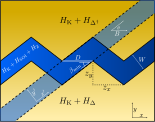
\includegraphics[width=0.75\columnwidth]{images/longest_trajectory_wo_corners}
			\caption{Diagram depicting quasiclassical estimate of a zigzag system, but now with the longest trajectory chosen to avoid the corners of the zigzag.}
			\label{fig:quasiclassical_approximation}
			\end{figure}

			\begin{figure}[!htb]
			\centering
			\includegraphics[width=0.95\columnwidth]{figures/z_y_vs_E_gap}
			\caption{Comparison of the topological gap computed using a full zigzag system implemented in Kwant with the quasiclassical estimate.
			The ratio $4\dfrac{z_x}{z_y}$ is kept constant at three different values, and the gap is calculated for varying $z_y$.
			The full lines represent  the numerical gap calculations of the full zigzag system, the dashed lines represent the quasiclassical estimation.}
			\label{fig:quasiclassical_approximation}
			\end{figure}

			We would expect that the maximum gap improvement would occur near where the zigzag amplitude $z_y$ is large enough to cut off any angle in the system.
			This point is different for the three ratios but can be identified by where the gap is largest for the quasiclassical estimate (dashed lines).
			Increasing $z_y$ further would only allow longer trajectories, which would seem extra undesirable due to the magnetic field not being aligned with the diagonal sections.

			Considering the lines corresponding to the full zigzag systems, we see that, for the lower ratios (and thus steeper slopes), the optimal value lies far beyond the cutoff point.
			This is unexpected, and it weakens the validity of the idea that the length of the trajectories mostly determines the gap.
			A possible explanation is that for lower ratios, the length of the diagonal sections is smaller, and it is easier for the wavefunction to tunnel through the superconductor.
			In any case, this phenomenon requires additional explanation.

			The quasiclassical estimate, indicated by the dashed lines, seems to underestimate the gap consistently.
			We also see that the gap declines monotonically with respect to the zigzag amplitude, which is by design: increasing the zigzag amplitude corresponds to increasing the domain of permitted trajectories, and thus the minimum can only decrease.
			Even so, we see that the decline of the gap with respect to $z_y$ is much quicker than with an actual zigzag.
			A possible reason that the quasiclassical model sketches a darker picture than full zigzag, is because in that model, long trajectories also correspond to grazing angles of incidence at the NS interface.

			We conclude that the proposed model to estimate the gap does not capture all the physics of the zigzag very well: the model merely gives a lower bound for the topological gap.

% -*- root: ./report.tex -*-
\chapter{Conclusion}\label{chap:conclusion}
In the model we study, the introduction of a zigzag geometry increases the topological gap by several orders of magnitude while simultaneously reducing the Majorana length.
Additionally, the breaking of a chiral symmetry brings the system from the BDI symmetry class into the D symmetry class, resulting in a cleaner topological phase.  % Bas: how is the symmetry broken?
Together, these improvements directly affect the robustness of the Majorana state, potentially bringing us closer to reliably create topological devices.

\comment{With the current quasiclassical analogy, we are not able to explain the improvements of zigzag.}
The current used quasiclassical analogy, applied in the most lenient form, is not able to fully explain the increased gap of a zigzag system.
Furthermore, numerical simulation points out that the optimal geometry does not always coincide with the minimal trajectory length.
It is therefore unsure whether the improvement of the gap can be fully attributed to the elimination of long trajectories, or if the arising phenomena are due to other mechanisms.
In any case, the improvements are stable under a wide range of parameters, and the topological gap varies gradually as a function of geometry, indicating the effect is not merely coincidental.
Further study should be devoted to isolating the working principle behind the improvements of the zigzag geometry.

\comment{Extensions: we omit several physical effects, disorder, electrostatics, etc.}
In the model used, we omit several physical effects, such as disorder, electrostatics, the orbital effect, etc.  % Bas: what is etc.? Leave it out or write out the other effects
Apart from experimental verification, further study is required to see whether the conclusions of this model are valid.  % Bas: waar komt de onzekerheid vandaan? Waarom is er meer verificatie nodig?

\comment{Current fabrication techniques seem compatible with the proposed geometry, and experimental verification should point out whether it holds up to its promise.}
Current fabrication techniques seem compatible with the proposed geometry, and experimental verification should point out whether it holds up to its promise.
We note that slight modifications to the geometry, for example, to ease measurement, should not have large implications on the physics.
Currently, experimental groups have already fabricated zigzag devices (e.g. the image on the cover of this thesis), and measurements are underway.

\comment{It would be interesting to study what geometry creates an optimal environment for Majorana modes to exist.}
We have studied sawtooth, snake-like, and offset sinusoidal modulation of the semiconductor region, but perhaps a more exotic shape will be optimal. % Bas: note that research in shape optimization is in progress (Andre)
A study optimizing the geometry for supporting Majoranas would be an interesting continuation.

%% Use letters for the chapter numbers of the appendices.
\appendix

%\input{appendix-a}

\bibliography{report}

\end{document}

